\section{Introdução}

O Método dos Elementos Finitos (FEM) é uma técnica numérica utilizada na solução aproximada de problemas descritos por equações diferenciais. Neste trabalho, o método é aplicado a problemas unidimensionais e seus resultados são comparados com aqueles obtidos pelo Método das Diferenças Finitas (FDM).

Neste trabalho, inicialmente, construiremos uma solução manufaturada para comparar as soluções obtidas por FEM e FDM com uma solução analítica conhecida, além de avaliar a convergência dos métodos para diferentes discretizações. Em seguida, estudaremos um capacitor composto por dois dielétricos, para o qual será obtida a forma fraca do problema e comparadas as soluções numéricas fornecidas pelos dois métodos.


\section{Atividade 01 -- Solução manufaturada}
\subsection{Definição da solução manufaturada}

Para avaliar a implementação dos métodos numéricos, foi definida uma solução analítica conhecida no intervalo \(x \in [0,1]\). A função escolhida foi

\[
u_e(x)=x^2e^x+\cos(3x).
\]

A partir dessa expressão, calcula-se a derivada segunda,

\[
u_e''(x)
=
(x^2+4x+2)e^x-9\cos(3x).
\]

Dessa forma, a função fonte utilizada no problema é

\[
f(x)
=
(x^2+4x+2)e^x-9\cos(3x).
\]

As condições de contorno são obtidas diretamente a partir da solução manufaturada:

\[
u(0)=u_e(0)=1,
\]

\[
u(1)=u_e(1)=e+\cos(3).
\]

\subsection{Formulação do problema}

A partir da solução manufaturada definida anteriormente, o problema considerado consiste em encontrar \(u(x)\) no intervalo \(x \in [0,1]\) tal que

\[
u_{,xx}=f(x),
\]

com

\[
f(x)
=
(x^2+4x+2)e^x-9\cos(3x).
\]

As condições de contorno são definidas a partir da própria solução exata \(u_e(x)\), resultando em

\[
u(0)=1,
\]

\[
u(1)=e+\cos(3).
\]

Dessa forma, a solução analítica conhecida do problema é

\[
u_e(x)=x^2e^x+\cos(3x),
\]

que será utilizada como referência para a avaliação das soluções numéricas obtidas pelos métodos FEM e FDM.

\subsection{Implementação pelo Método dos Elementos Finitos}

Para a solução pelo Método dos Elementos Finitos, o domínio \(x \in [0,1]\) foi discretizado em elementos unidimensionais lineares. Partindo da equação

\[
u_{,xx}=f(x),
\]

multiplica-se ambos os lados por uma função de ponderação \(w(x)\) e integra-se sobre o domínio:

\[
\int_0^1 w\,u_{,xx}\,dx
=
\int_0^1 w\,f\,dx.
\]

Aplicando integração por partes, obtém-se

\[
\left[w\,u_{,x}\right]_0^1
-
\int_0^1 w_{,x}u_{,x}\,dx
=
\int_0^1 w\,f\,dx.
\]

Como as condições de contorno são prescritas nas duas extremidades, as funções de ponderação são nulas em \(x=0\) e \(x=1\). Dessa forma, a forma fraca do problema pode ser escrita como

\[
\int_0^1 w_{,x}u_{,x}\,dx
=
-
\int_0^1 w\,f\,dx.
\]

A solução aproximada é construída utilizando funções de forma lineares em cada elemento. A aplicação do método de Galerkin resulta em um sistema linear da forma

\[
K\mathbf{u}=\mathbf{F},
\]

em que \(K\) representa a matriz global associada às derivadas das funções de forma e \(\mathbf{F}\) representa o vetor correspondente à função fonte.

Após a montagem do sistema, são impostas as condições de contorno

\[
u(0)=1,
\]

\[
u(1)=1+e,
\]

e o sistema resultante é resolvido para determinar os valores aproximados da solução nos nós da malha.

\subsection{Implementação pelo Método das Diferenças Finitas}

Para a solução pelo Método das Diferenças Finitas, o domínio \(x \in [0,1]\) foi discretizado em pontos igualmente espaçados. A derivada segunda foi aproximada por diferenças centrais de segunda ordem,

\[
u_{,xx}(x_i)
\approx
\frac{u_{i-1}-2u_i+u_{i+1}}{h^2},
\]

em que \(h\) representa o espaçamento entre os pontos da malha.

Substituindo essa aproximação na equação diferencial

\[
u_{,xx}=f(x),
\]

obtém-se, para os pontos internos,

\[
\frac{u_{i-1}-2u_i+u_{i+1}}{h^2}
=
f(x_i).
\]

Reorganizando a expressão,

\[
u_{i-1}-2u_i+u_{i+1}
=
h^2 f(x_i).
\]

A aplicação dessa equação em todos os pontos internos do domínio resulta em um sistema linear para os valores aproximados de \(u\). As condições de contorno

\[
u(0)=1
\]

e

\[
u(1)=1+e
\]

são incorporadas ao sistema, permitindo calcular a solução numérica nos pontos da malha.

\subsection{Comparação das soluções para \(n=6\)}

Para comparar os métodos numéricos, foram calculadas as soluções pelo Método dos Elementos Finitos e pelo Método das Diferenças Finitas utilizando \(n=6\) pontos internos. Em ambos os casos, os resultados foram comparados com a solução analítica

\[
u_e(x)=x^2e^x+\cos(3x).
\]

A Figura~\ref{fig:comparacao_n6} apresenta a comparação entre as soluções obtidas pelos dois métodos e a solução analítica.

\begin{figure}[H]
    \centering
    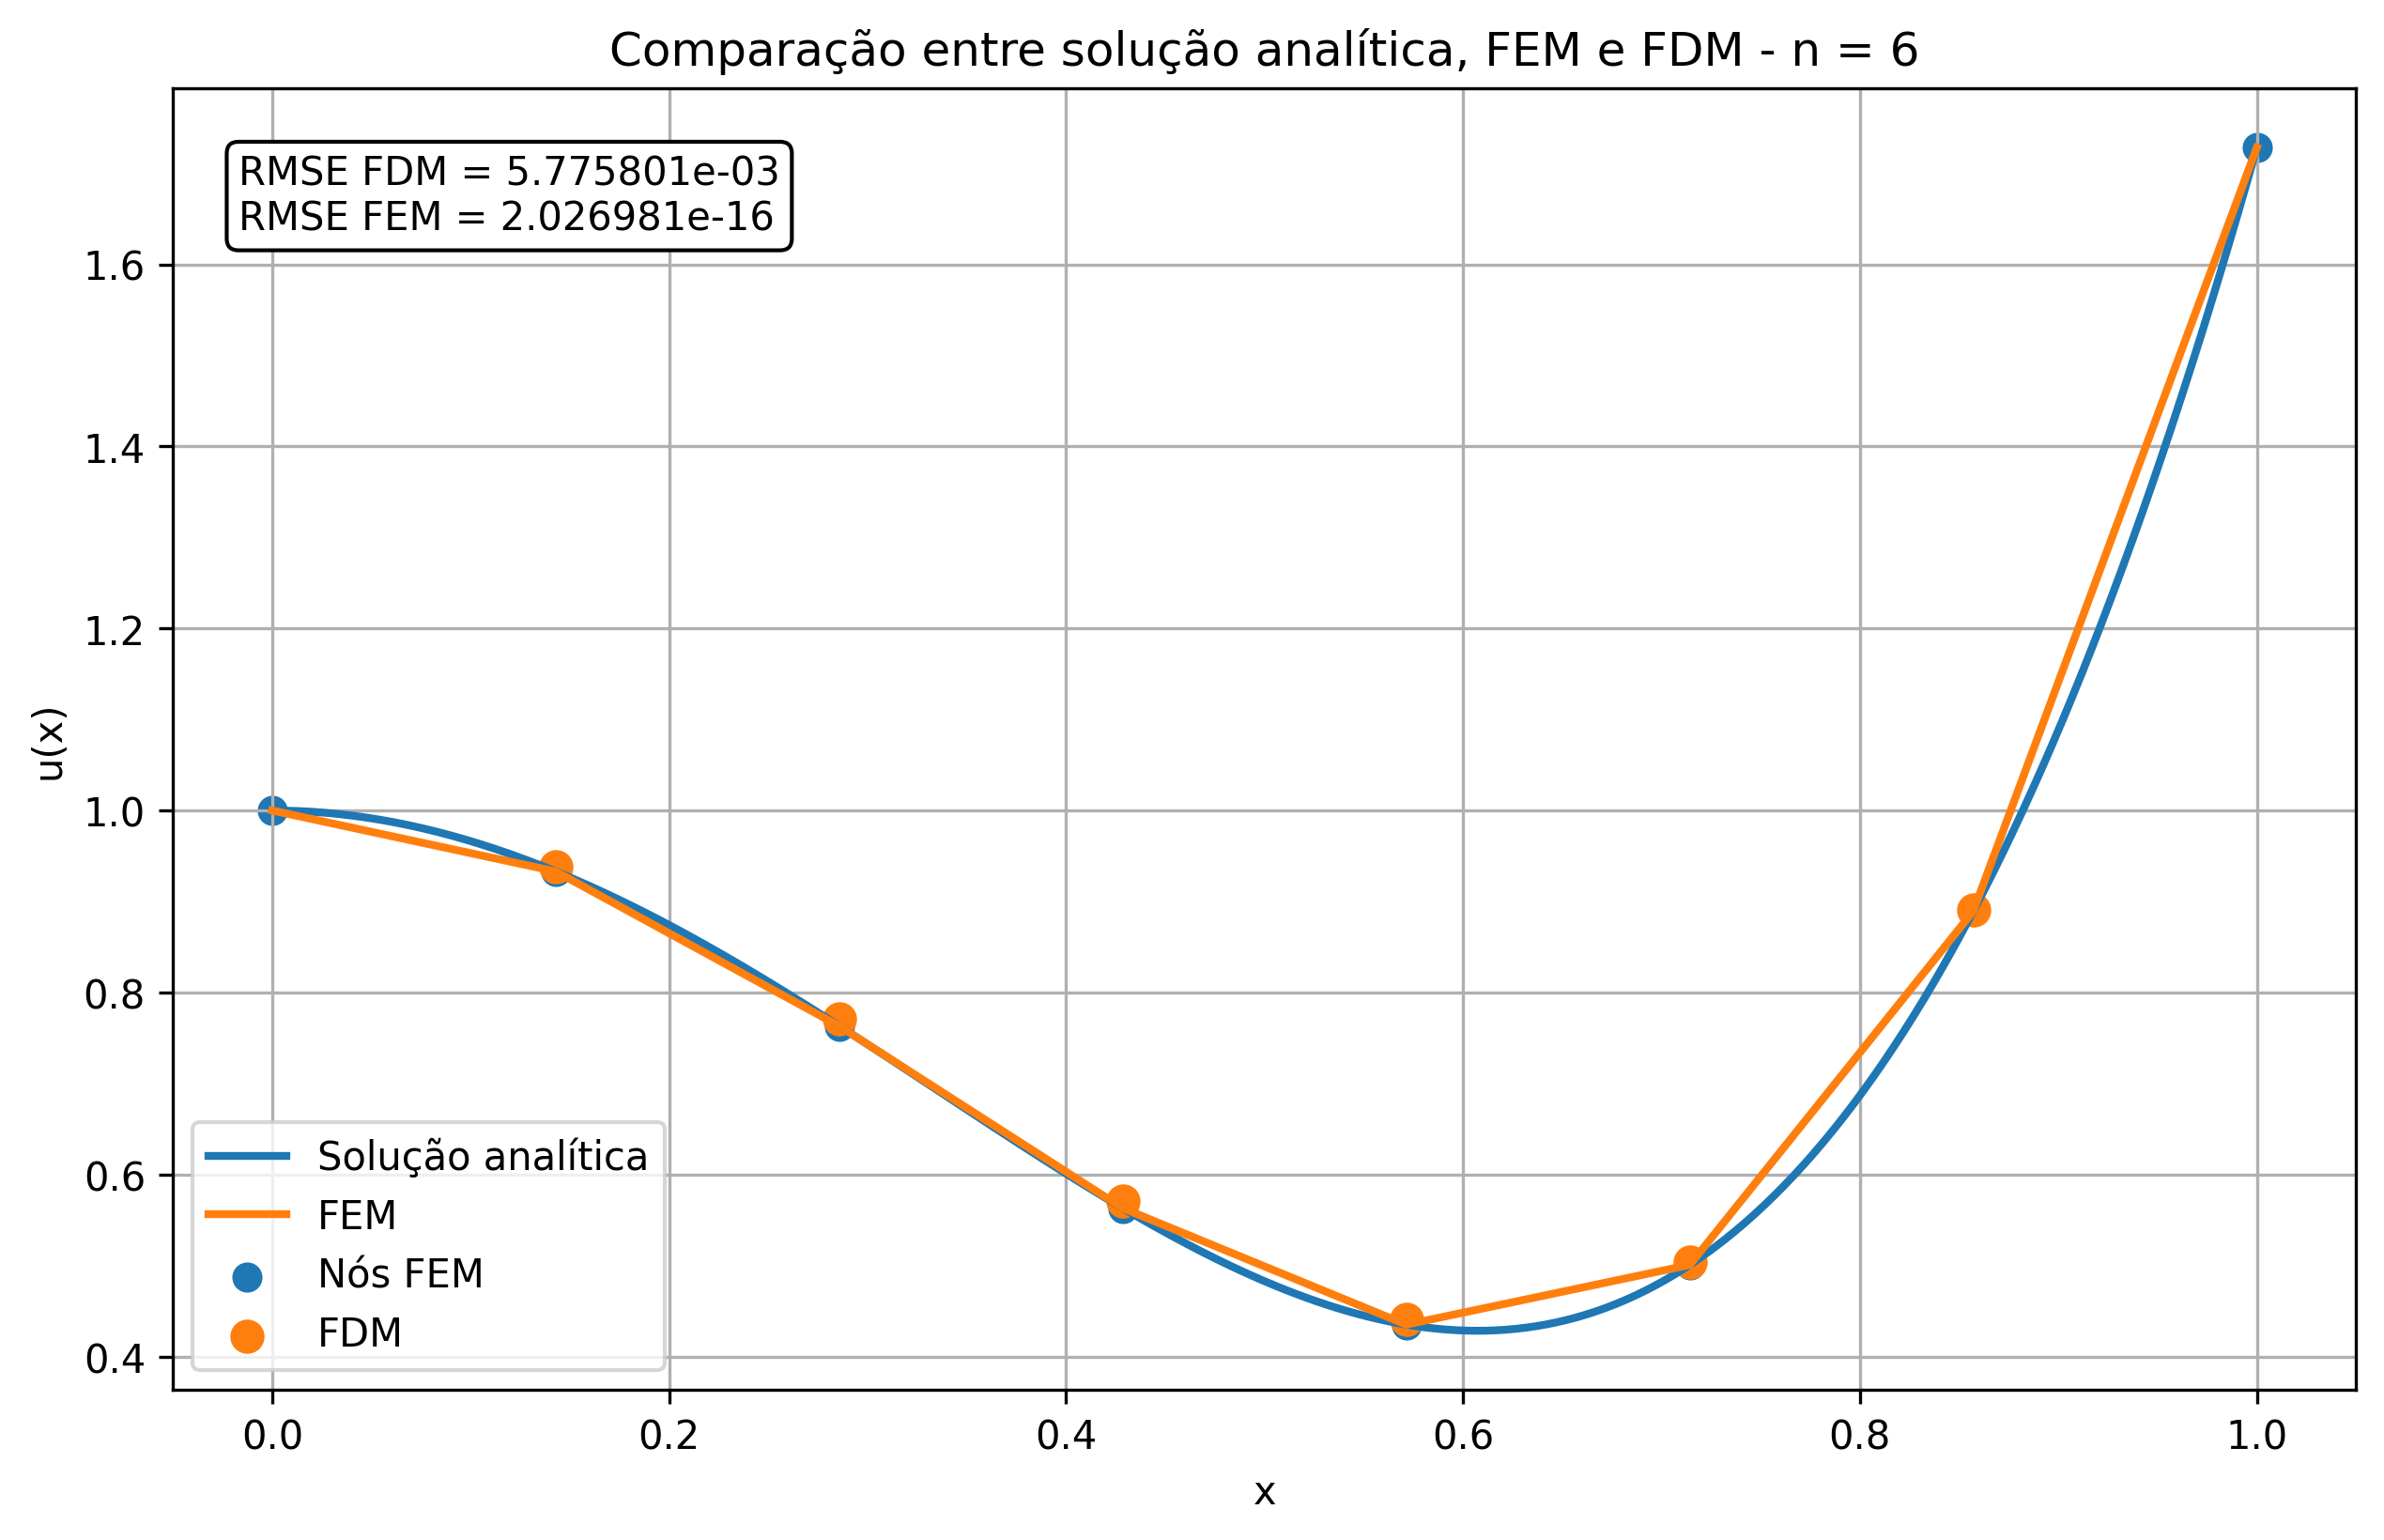
\includegraphics[width=0.85\textwidth]{imagens/comparacao_n6.png}
    \caption{Comparação entre a solução analítica e as soluções obtidas pelos métodos FEM e FDM para \(n=6\).}
    \label{fig:comparacao_n6}
\end{figure}

Para o Método das Diferenças Finitas, o erro médio quadrático obtido foi

\[
\mathrm{RMSE}_{\mathrm{FDM}}
=
5{,}776\times10^{-3}.
\]

Para o Método dos Elementos Finitos, considerando o erro calculado nos nós internos da malha, foi obtido

\[
\mathrm{RMSE}_{\mathrm{FEM}}
=
2{,}027\times10^{-16}.
\]

Observa-se que ambos os métodos apresentam boa aproximação da solução analítica. No FEM, os valores obtidos nos nós praticamente coincidem com a solução exata, enquanto entre os nós a solução é representada por funções lineares por partes. O FDM também acompanha adequadamente a solução analítica, embora apresente um erro nodal superior ao observado no FEM para essa discretização.

A influência do refinamento da malha sobre os erros dos dois métodos será analisada na seção seguinte.

\subsection{Análise de convergência}

Para avaliar a convergência dos métodos numéricos, foram consideradas diferentes discretizações do domínio, utilizando

\[
n=4,\;8,\;16,\;32.
\]

Para cada valor de \(n\), foram calculadas as soluções pelos métodos FEM e FDM e determinado o erro médio quadrático em relação à solução analítica \(u_e(x)\).

Na comparação apresentada anteriormente para \(n=6\), o erro do FEM foi calculado apenas nos nós internos da malha, resultando em um valor praticamente nulo. Entretanto, esse resultado representa apenas o erro nodal e não considera as diferenças existentes entre a solução analítica e a aproximação linear do FEM no interior de cada elemento.

Por esse motivo, para a análise de convergência, as soluções numéricas dos métodos FEM e FDM foram interpoladas linearmente sobre uma mesma malha de avaliação composta por 2001 pontos uniformemente distribuídos no intervalo \([0,1]\). Dessa forma, o erro foi avaliado ao longo de todo o domínio utilizando o mesmo conjunto de pontos para os dois métodos.

O erro médio quadrático utilizado na comparação foi definido por

\[
\mathrm{RMSE}
=
\sqrt{
\frac{1}{N}
\sum_{i=1}^{N}
\left(
u_i-u_e(x_i)
\right)^2
},
\]

em que \(u_i\) representa a solução numérica interpolada no ponto \(x_i\), \(u_e(x_i)\) corresponde à solução analítica e \(N\) representa o número de pontos utilizados na avaliação do erro.

Os resultados obtidos são apresentados na Tabela~\ref{tab:convergencia}.

\begin{table}[H]
    \centering
    \caption{Erro médio quadrático dos métodos FEM e FDM para diferentes discretizações.}
    \label{tab:convergencia}
    \begin{tabular}{c c c c}
        \hline
        \(n\) & \(h\) & RMSE FEM & RMSE FDM \\
        \hline
        4  & 0,200000 & \(4,8389\times10^{-2}\) & \(5,1962\times10^{-2}\) \\
        8  & 0,111111 & \(1,5051\times10^{-2}\) & \(1,6131\times10^{-2}\) \\
        16 & 0,058824 & \(4,2290\times10^{-3}\) & \(4,5297\times10^{-3}\) \\
        32 & 0,030303 & \(1,1231\times10^{-3}\) & \(1,2027\times10^{-3}\) \\
        \hline
    \end{tabular}
\end{table}

A Figura~\ref{fig:convergencia} apresenta a evolução do erro em função do refinamento da malha.

\begin{figure}[H]
    \centering
    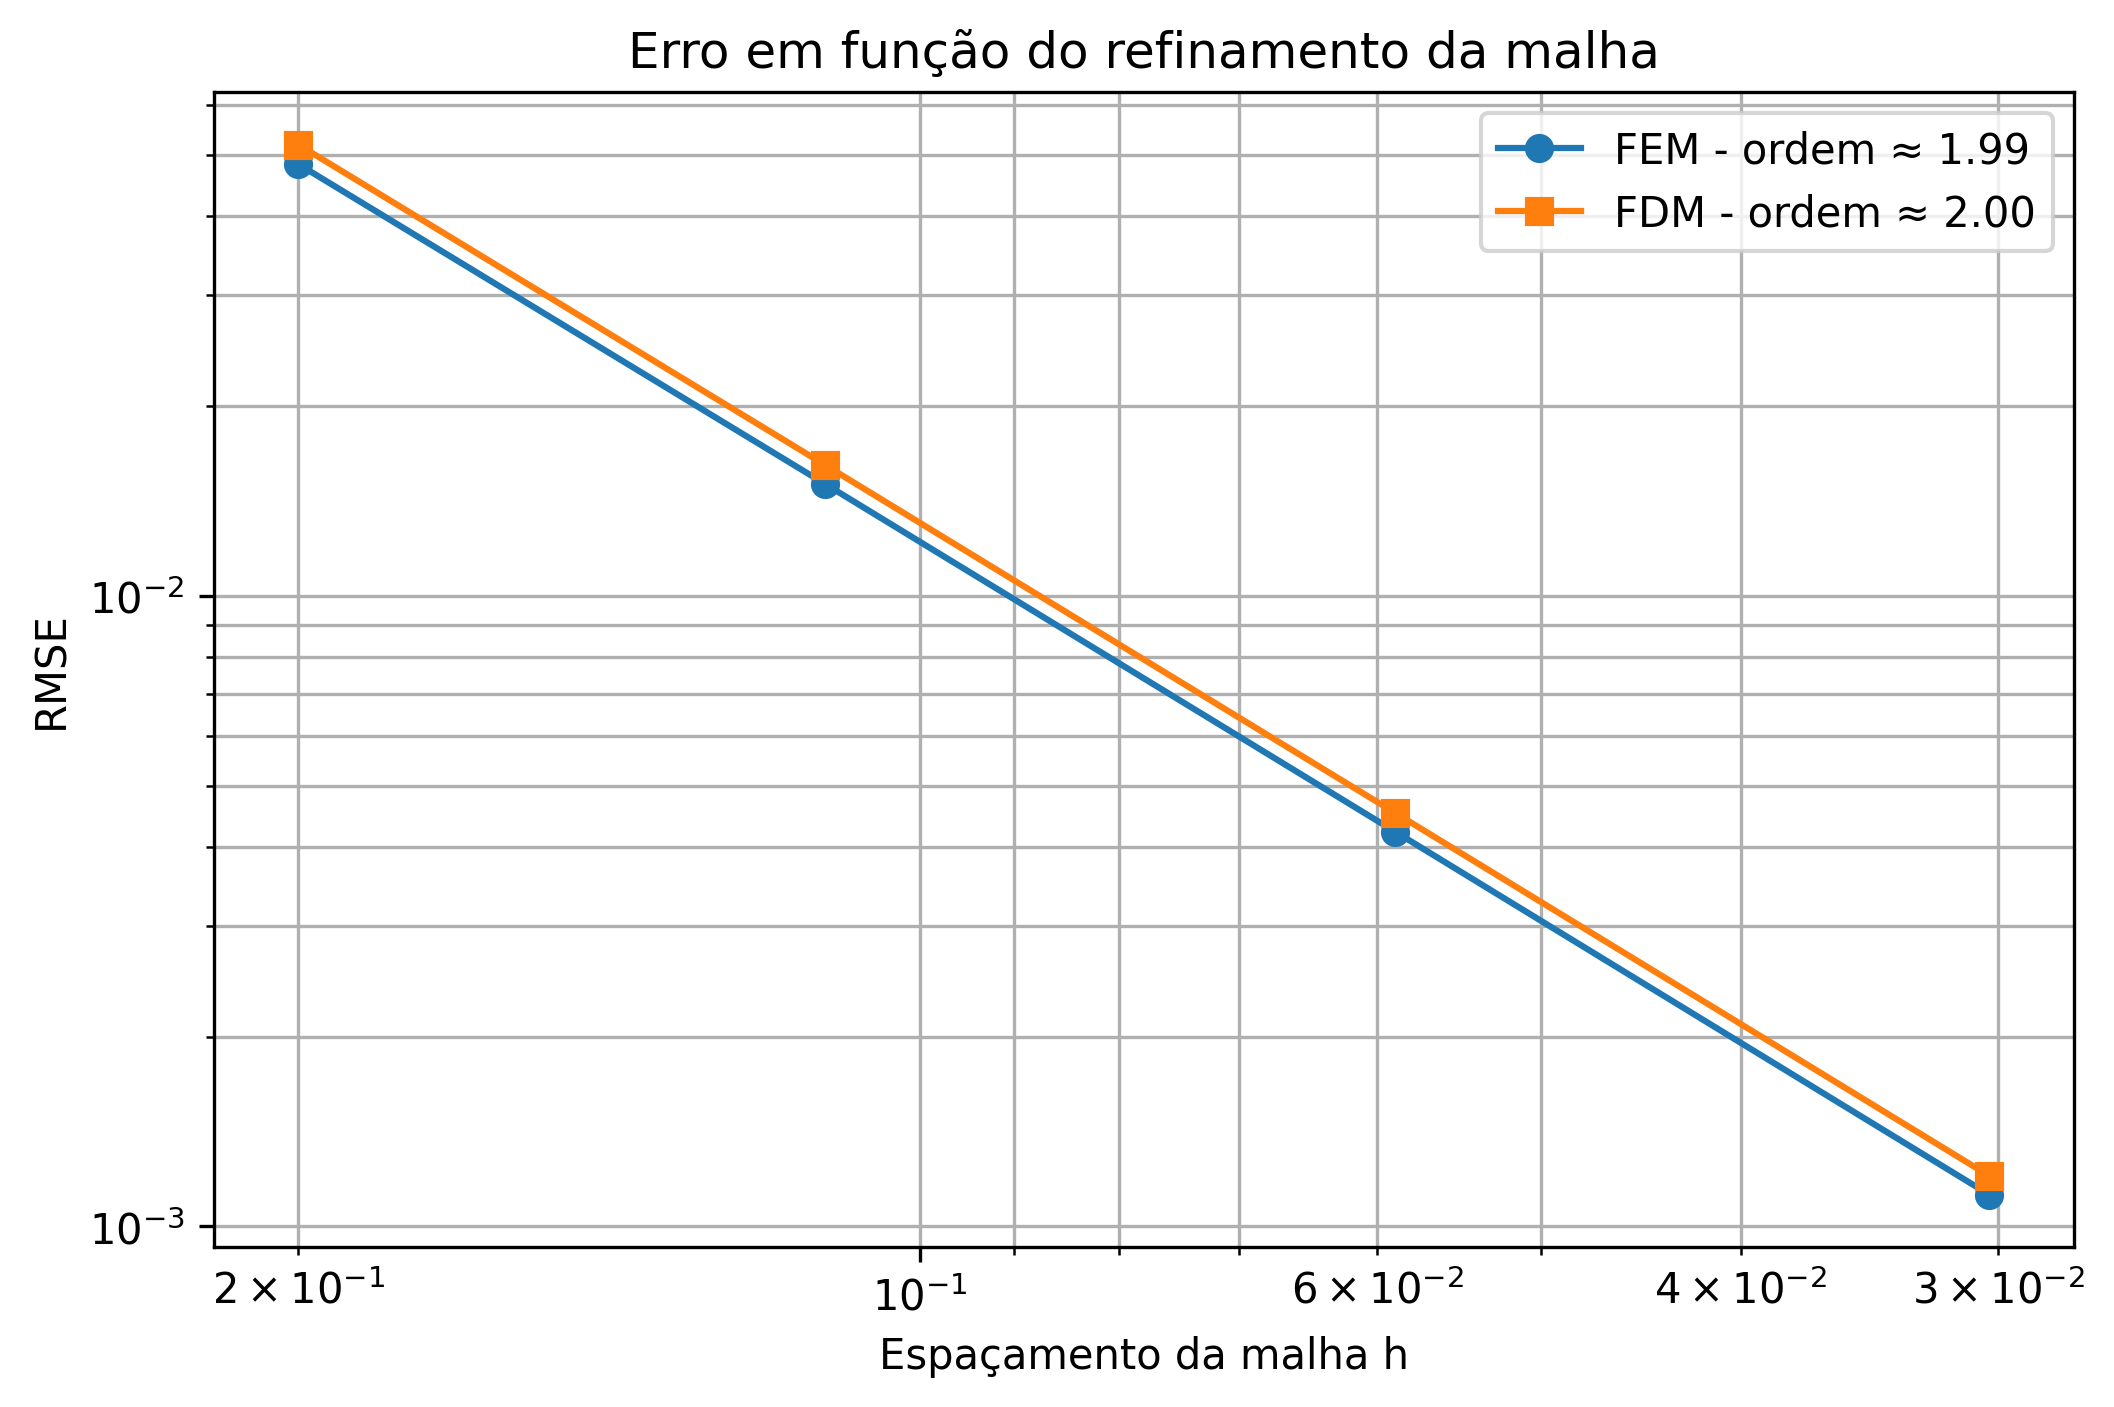
\includegraphics[width=0.80\textwidth]{imagens/convergencia_h.png}
    \caption{Erro médio quadrático em função do espaçamento da malha para os métodos FEM e FDM.}
    \label{fig:convergencia}
\end{figure}

Observa-se uma redução sistemática do erro à medida que a malha é refinada para ambos os métodos. O FEM apresentou valores de RMSE ligeiramente inferiores aos obtidos pelo FDM em todas as discretizações analisadas.

A partir da relação entre o erro e o espaçamento da malha, foram estimadas ordens de convergência de aproximadamente

\[
p_{\mathrm{FEM}} \approx 1,99
\]

e

\[
p_{\mathrm{FDM}} \approx 2,00.
\]

Esses resultados indicam comportamento aproximadamente de segunda ordem para os dois métodos na solução do problema considerado.

\subsection{Discussão dos resultados}

Os resultados obtidos mostram que os métodos FEM e FDM foram capazes de aproximar adequadamente a solução analítica do problema manufaturado. Para \(n=6\), ambos apresentaram boa concordância com a solução exata, sendo observado erro nodal praticamente nulo para o FEM e um pequeno erro para o FDM.

Na análise de convergência, o refinamento da malha resultou em redução sistemática do erro para os dois métodos. As ordens estimadas, próximas de 2, indicam comportamento de segunda ordem tanto para o FEM quanto para o FDM no problema considerado.

De forma geral, os resultados confirmam a consistência das implementações e mostram que ambas as abordagens convergem para a solução analítica à medida que a discretização é refinada.

\section{Atividade 02 -- Capacitor composto por dois dielétricos}

\subsection{Formulação do problema}

Nesta atividade, considera-se um capacitor composto por dois materiais dielétricos distintos ao longo do domínio unidimensional

\[
\Omega = (0,L).
\]

O potencial elétrico \(\phi(z)\) deve satisfazer a equação

\[
\frac{d}{dz}
\left(
\varepsilon_r(z)
\frac{d\phi(z)}{dz}
\right)
=0,
\]

com as condições de contorno

\[
\phi(0)=V_a,
\]

\[
\phi(L)=V_b.
\]

Para o problema considerado, são utilizados os parâmetros

\[
L=1,
\qquad
V_a=10,
\qquad
V_b=0.
\]

A permissividade relativa varia ao longo do domínio de acordo com

\[
\varepsilon_r(z)=
\begin{cases}
3, & z < \dfrac{L}{2},\\[6pt]
1, & z \geq \dfrac{L}{2}.
\end{cases}
\]

Dessa forma, o domínio é dividido em duas regiões com diferentes propriedades dielétricas, cuja interface está localizada em

\[
z=\frac{L}{2}=0{,}5.
\]

A Figura~\ref{fig:permissividade_capacitor} apresenta a distribuição da permissividade relativa ao longo do domínio, evidenciando a descontinuidade existente na interface entre os dois materiais.

\begin{figure}[H]
    \centering
    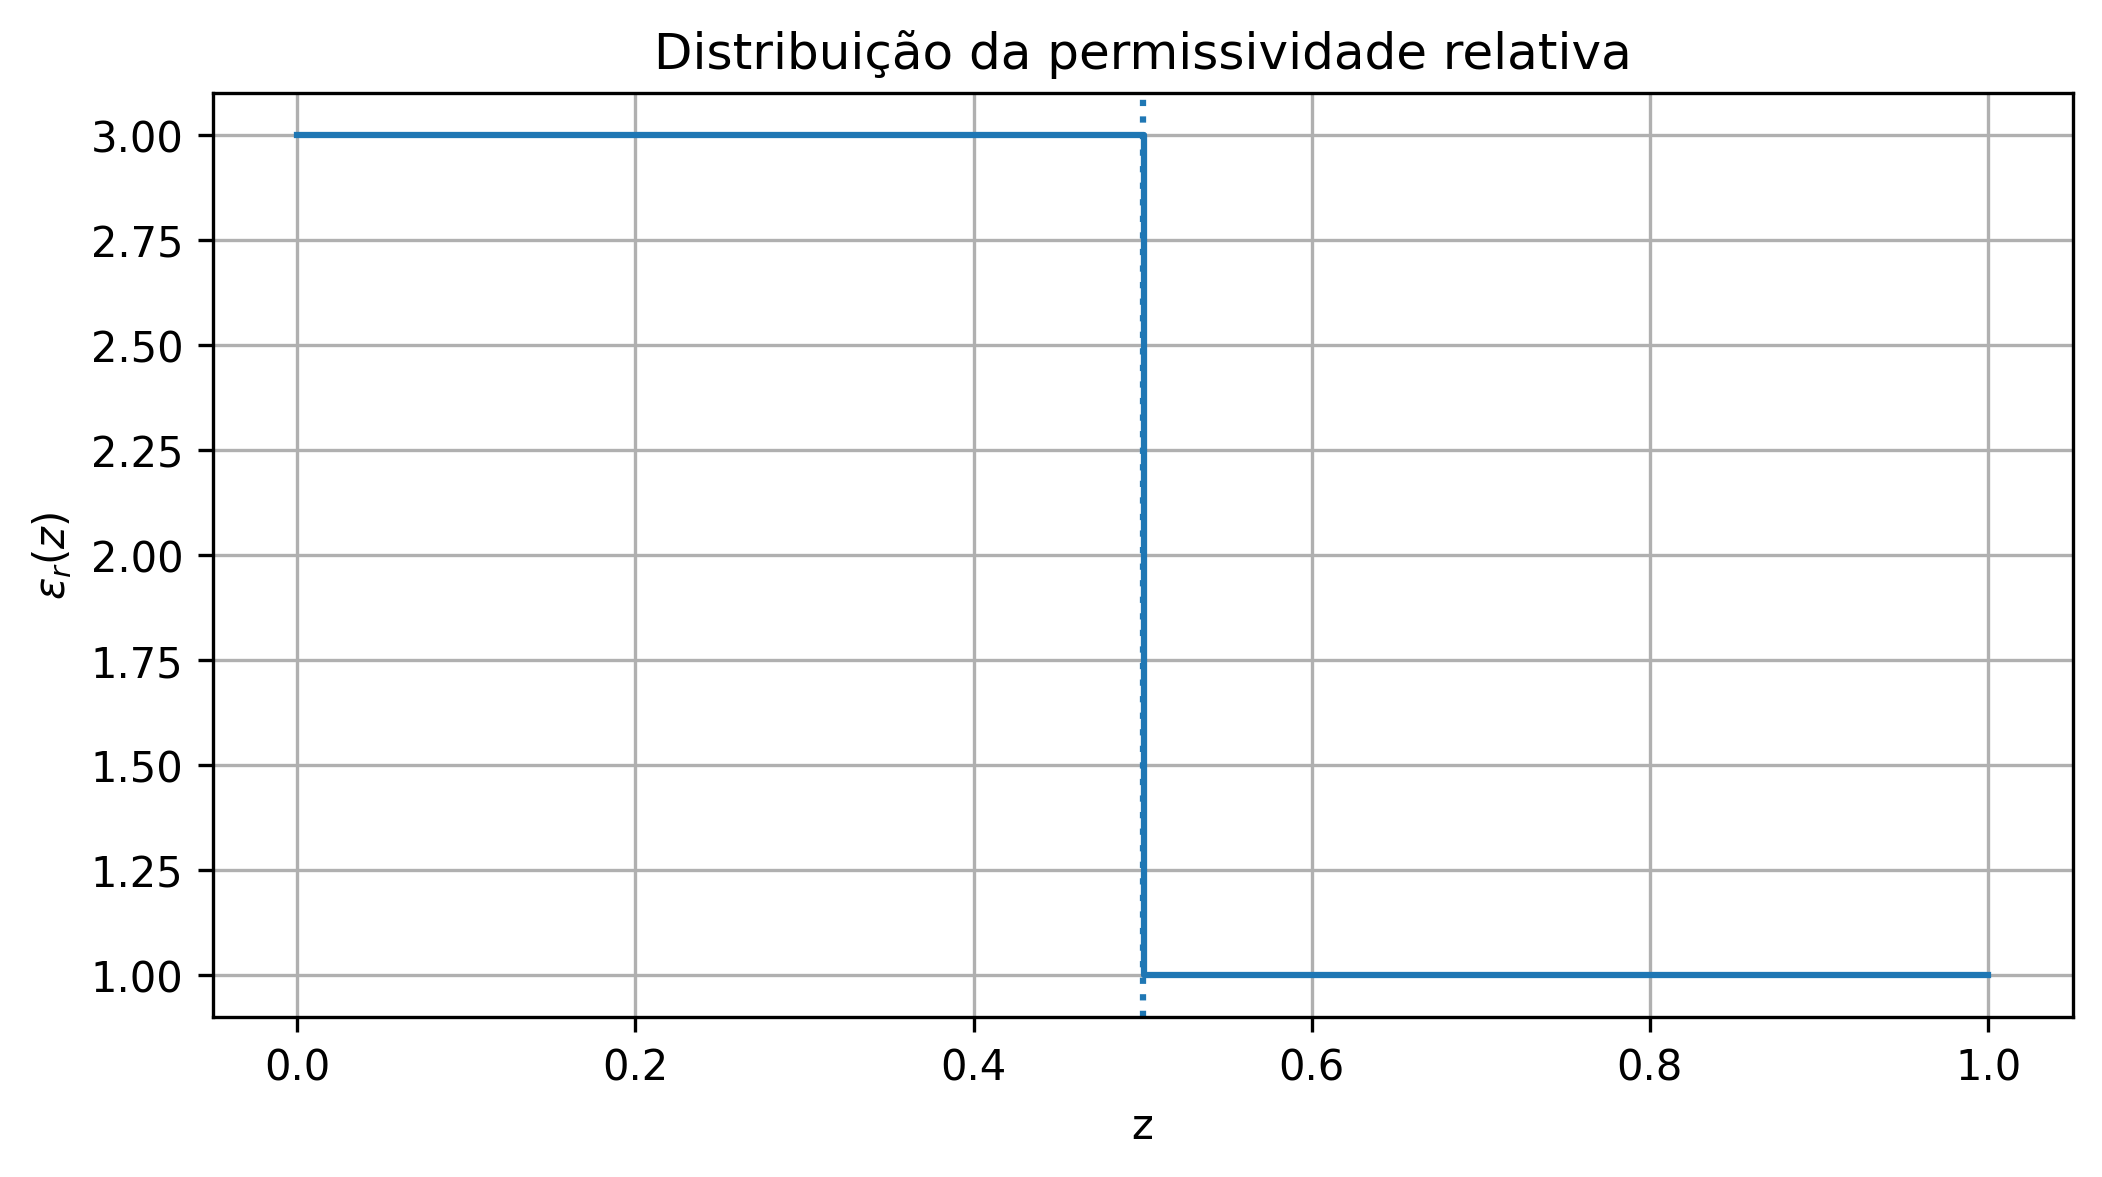
\includegraphics[width=0.75\textwidth]{imagens/permissividade_capacitor.png}
    \caption{Distribuição da permissividade relativa ao longo do domínio do capacitor.}
    \label{fig:permissividade_capacitor}
\end{figure}

\subsection{Obtenção da forma fraca}

Partindo da equação diferencial

\[
\frac{d}{dz}
\left(
\varepsilon_r(z)
\frac{d\phi}{dz}
\right)
=0,
\]

multiplica-se ambos os lados por uma função de ponderação \(w(z)\) e integra-se sobre o domínio.

Como a permissividade relativa assume valores constantes em cada região, o domínio é dividido em duas partes:

\[
\int_{0}^{L/2}
w
\frac{d}{dz}
\left(
\varepsilon_1
\frac{d\phi}{dz}
\right)
dz
+
\int_{L/2}^{L}
w
\frac{d}{dz}
\left(
\varepsilon_2
\frac{d\phi}{dz}
\right)
dz
=0,
\]

em que

\[
\varepsilon_1=3
\]

e

\[
\varepsilon_2=1.
\]

Aplicando integração por partes em cada uma das integrais, obtém-se

\[
\left[
w\varepsilon_1\frac{d\phi}{dz}
\right]_{0}^{L/2}
-
\int_{0}^{L/2}
\varepsilon_1
\frac{dw}{dz}
\frac{d\phi}{dz}
\,dz
\]

\[
+
\left[
w\varepsilon_2\frac{d\phi}{dz}
\right]_{L/2}^{L}
-
\int_{L/2}^{L}
\varepsilon_2
\frac{dw}{dz}
\frac{d\phi}{dz}
\,dz
=0.
\]

Como as condições de contorno de Dirichlet são prescritas em \(z=0\) e \(z=L\), as funções de ponderação satisfazem

\[
w(0)=0,
\qquad
w(L)=0.
\]

Além disso, na interface entre os dois dielétricos é imposta a continuidade do fluxo elétrico,

\[
\varepsilon_1
\left.
\frac{d\phi}{dz}
\right|_{L/2^-}
=
\varepsilon_2
\left.
\frac{d\phi}{dz}
\right|_{L/2^+}.
\]

Dessa forma, os termos de contorno na interface se cancelam e a forma fraca do problema pode ser escrita como

\[
\int_{0}^{L/2}
\varepsilon_1
\frac{dw}{dz}
\frac{d\phi}{dz}
\,dz
+
\int_{L/2}^{L}
\varepsilon_2
\frac{dw}{dz}
\frac{d\phi}{dz}
\,dz
=0.
\]

Equivalentemente, utilizando a função \(\varepsilon_r(z)\), obtém-se

\[
\int_{0}^{L}
\varepsilon_r(z)
\frac{dw}{dz}
\frac{d\phi}{dz}
\,dz
=0.
\]

\subsection{Implementação pelo Método dos Elementos Finitos}

Para a solução pelo Método dos Elementos Finitos, o domínio foi discretizado em elementos unidimensionais lineares, de forma que exista um nó exatamente na interface entre os dois dielétricos,

\[
z=\frac{L}{2}=0{,}5.
\]

Para isso, foi adotado um número ímpar de nós, conforme solicitado no enunciado.

A partir da forma fraca,

\[
\int_{0}^{L}
\varepsilon_r(z)
\frac{dw}{dz}
\frac{d\phi}{dz}
\,dz
=0,
\]

a contribuição de cada elemento para a matriz de rigidez é dada por

\[
K^{(e)}
=
\int_{\Omega_e}
\varepsilon_r
\mathbf{B}^{T}\mathbf{B}
\,dz,
\]

em que \(\mathbf{B}\) contém as derivadas das funções de forma lineares do elemento.

Para um elemento de comprimento \(h_e\), com permissividade relativa constante \(\varepsilon_r^{(e)}\), a matriz local pode ser escrita como

\[
K^{(e)}
=
\frac{\varepsilon_r^{(e)}}{h_e}
\begin{bmatrix}
1 & -1 \\
-1 & 1
\end{bmatrix}.
\]

A matriz global é obtida pela montagem das contribuições de todos os elementos, utilizando \(\varepsilon_r=3\) nos elementos localizados na primeira metade do domínio e \(\varepsilon_r=1\) nos elementos da segunda metade.

Após a montagem do sistema, são impostas as condições de contorno

\[
\phi(0)=10
\]

e

\[
\phi(1)=0.
\]

A solução do sistema linear resultante fornece os valores aproximados do potencial elétrico nos nós da malha.

\subsection{Implementação pelo Método das Diferenças Finitas}

Para a solução pelo Método das Diferenças Finitas, o domínio foi discretizado em pontos igualmente espaçados, incluindo um ponto exatamente na interface entre os dois dielétricos,

\[
z=\frac{L}{2}=0{,}5.
\]

A equação diferencial considerada é

\[
\frac{d}{dz}
\left(
\varepsilon_r(z)
\frac{d\phi}{dz}
\right)
=0.
\]

Como a permissividade relativa varia ao longo do domínio, a discretização é realizada considerando os valores de \(\varepsilon_r\) entre os pontos da malha. Para um ponto interno \(z_i\), a equação discretizada pode ser escrita como

\[
\frac{1}{h}
\left[
\varepsilon_{i+\frac{1}{2}}
\frac{\phi_{i+1}-\phi_i}{h}
-
\varepsilon_{i-\frac{1}{2}}
\frac{\phi_i-\phi_{i-1}}{h}
\right]
=0,
\]

em que \(h\) representa o espaçamento da malha e
\(\varepsilon_{i\pm\frac{1}{2}}\) correspondem aos valores de permissividade entre os pontos adjacentes.

Reorganizando a expressão, obtém-se

\[
-\varepsilon_{i-\frac{1}{2}}\phi_{i-1}
+
\left(
\varepsilon_{i-\frac{1}{2}}
+
\varepsilon_{i+\frac{1}{2}}
\right)\phi_i
-
\varepsilon_{i+\frac{1}{2}}\phi_{i+1}
=0.
\]

A aplicação dessa equação nos pontos internos resulta em um sistema linear para os valores do potencial elétrico. As condições de contorno

\[
\phi(0)=10
\]

e

\[
\phi(1)=0
\]

são incorporadas ao sistema antes de sua solução.

\subsection{Comparação dos resultados}

As soluções obtidas pelos métodos FEM e FDM foram comparadas utilizando uma malha com nove nós, incluindo um nó localizado exatamente na interface entre os dois dielétricos,

\[
z=\frac{L}{2}=0{,}5.
\]

A Figura~\ref{fig:comparacao_capacitor} apresenta a distribuição do potencial elétrico obtida pelos dois métodos.

\begin{figure}[H]
    \centering
    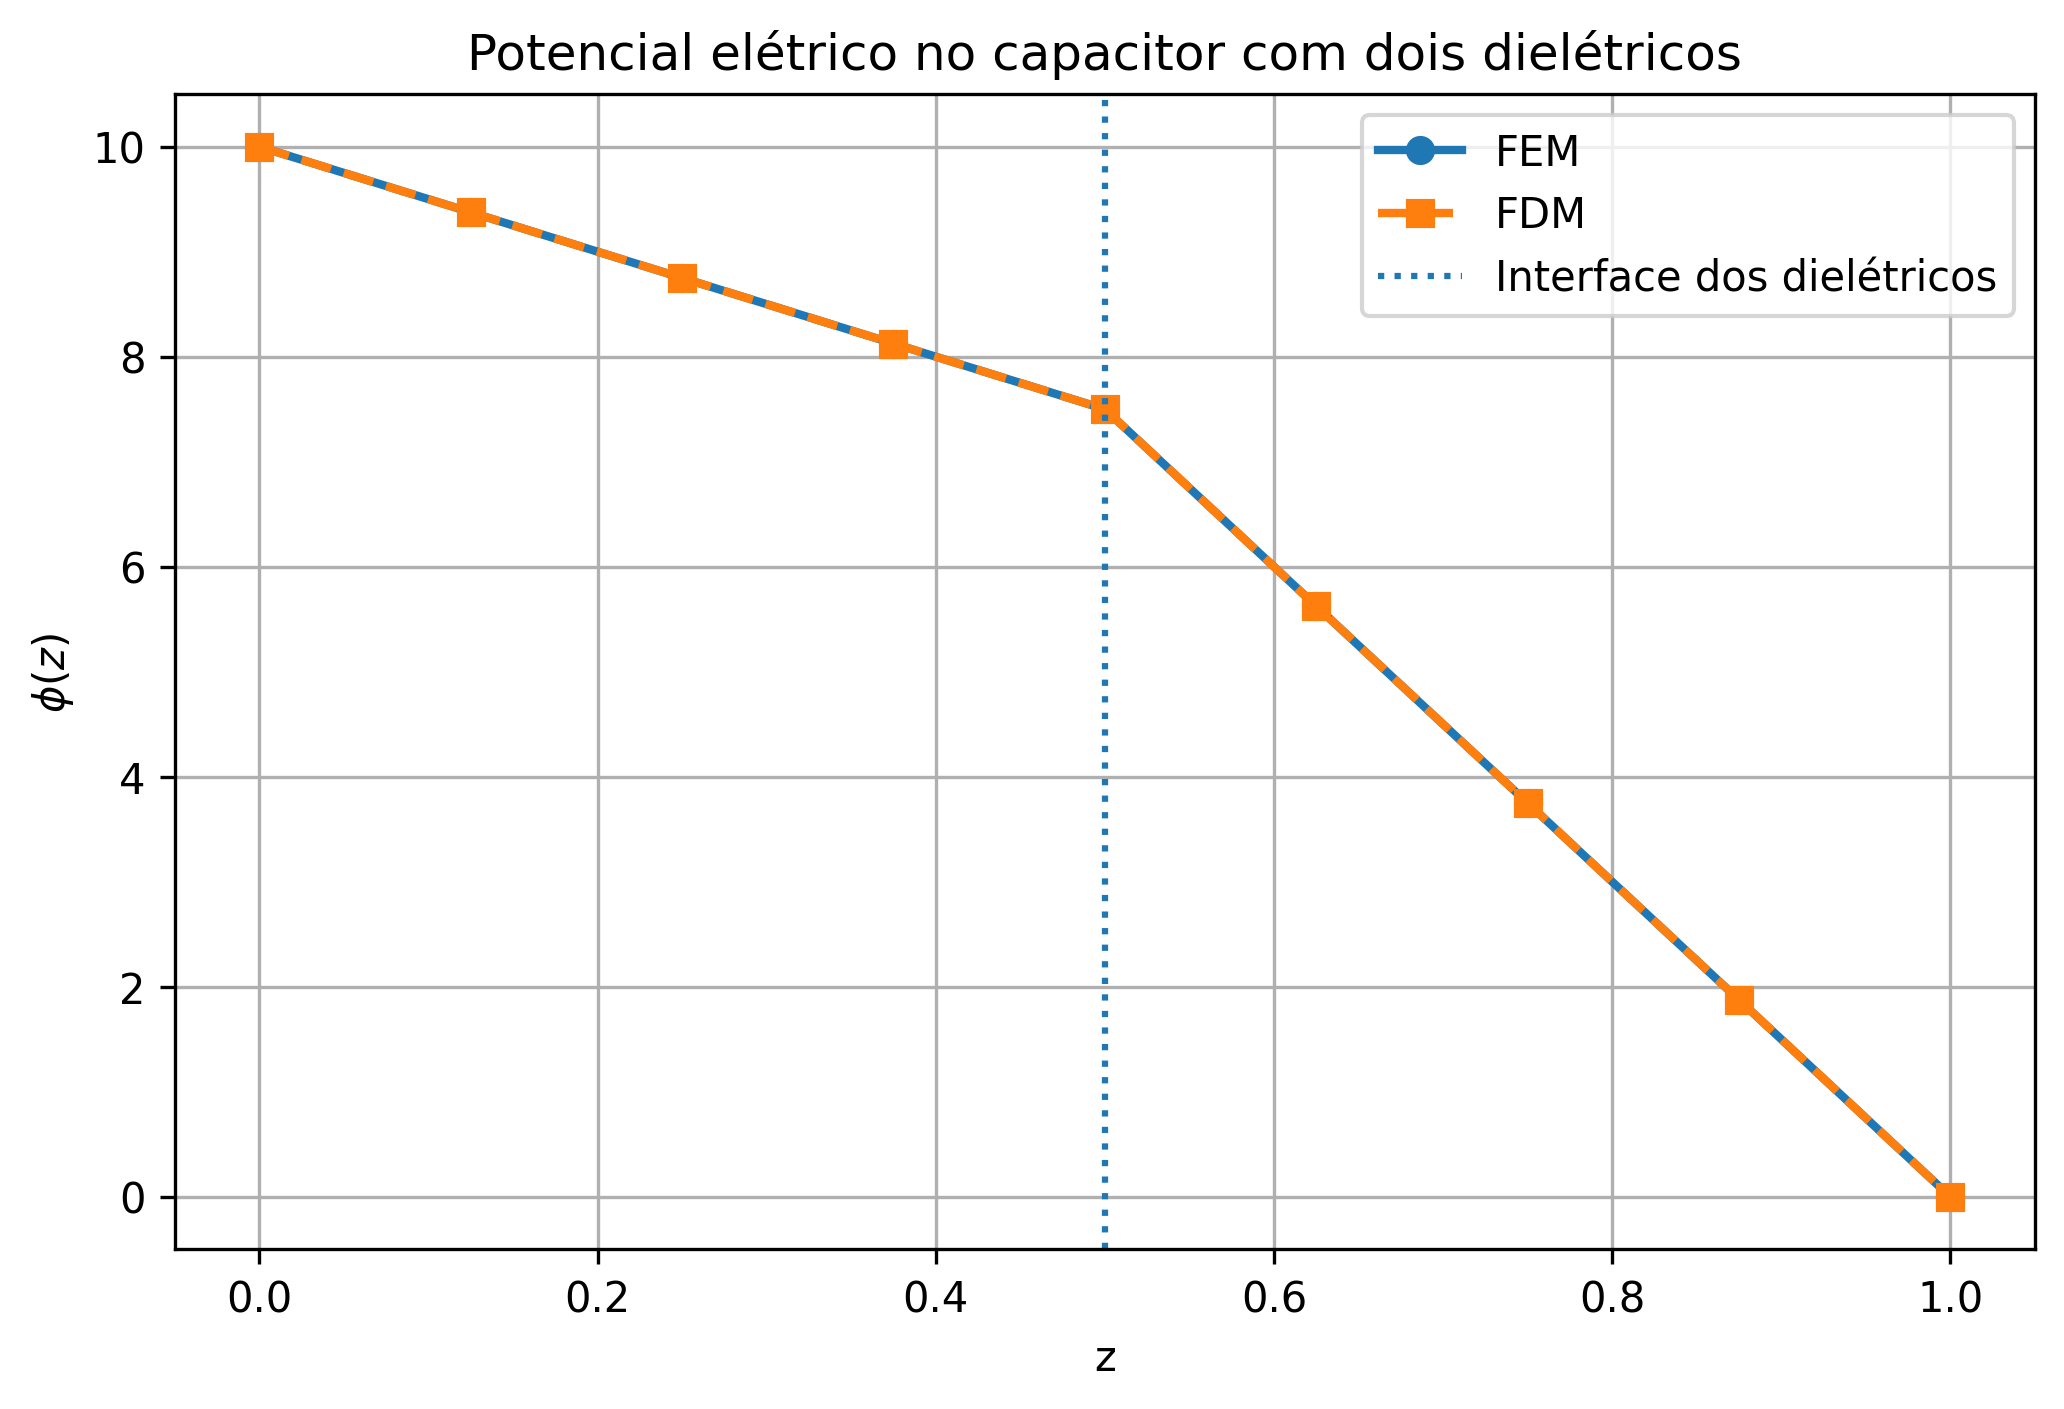
\includegraphics[width=0.85\textwidth]{imagens/comparacao_capacitor.png}
    \caption{Comparação entre as soluções obtidas pelos métodos FEM e FDM para o capacitor composto por dois dielétricos.}
    \label{fig:comparacao_capacitor}
\end{figure}

Os dois métodos forneceram os mesmos valores de potencial nos pontos da malha. Na interface entre os dielétricos, foi obtido

\[
\phi(0{,}5)=7{,}5,
\]

tanto para o FEM quanto para o FDM. A diferença máxima observada entre as duas soluções foi numericamente nula.

Observa-se que o potencial permanece contínuo em todo o domínio, mas apresenta uma mudança de inclinação na interface entre os materiais. Na região em que \(\varepsilon_r=3\), o potencial varia mais lentamente, enquanto na região em que \(\varepsilon_r=1\) a variação é mais acentuada.

O fluxo

\[
\varepsilon_r\frac{d\phi}{dz}
\]

foi calculado em cada elemento, apresentando valor constante igual a

\[
\varepsilon_r\frac{d\phi}{dz}=-15.
\]

Esse resultado confirma a continuidade do fluxo elétrico através da interface entre os dois dielétricos.

\subsection{Discussão dos resultados}

Os resultados obtidos para o capacitor composto por dois dielétricos mostraram concordância entre as soluções calculadas pelos métodos FEM e FDM. Para a malha utilizada, os valores de potencial obtidos pelos dois métodos coincidiram em todos os nós, incluindo a interface entre os materiais, onde foi encontrado

\[
\phi(0{,}5)=7{,}5.
\]

A distribuição do potencial apresentou comportamento linear em cada região, com mudança de inclinação na interface entre os dielétricos. Essa mudança está diretamente associada à diferença entre os valores de permissividade relativa dos materiais.

Também foi verificado que a grandeza

\[
\varepsilon_r\frac{d\phi}{dz}
\]

permaneceu constante ao longo de todo o domínio, com valor igual a

\[
-15.
\]

Esse resultado confirma a continuidade do fluxo elétrico na interface e mostra que a discretização adotada representou adequadamente a transição entre os dois meios materiais.

De forma geral, os resultados indicam que os métodos FEM e FDM fornecem soluções equivalentes para o problema considerado quando a interface entre os dielétricos coincide com um ponto da malha.

\section{Conclusão}

O presente trabalho permitiu aplicar e comparar os métodos de Elementos Finitos e Diferenças Finitas na solução de problemas unidimensionais.

Na primeira atividade, a utilização de uma solução manufaturada possibilitou avaliar diretamente a precisão dos métodos. Os resultados mostraram boa concordância com a solução analítica e comportamento de convergência aproximadamente de segunda ordem para FEM e FDM à medida que a malha foi refinada.

Na segunda atividade, os dois métodos foram aplicados ao problema de um capacitor composto por dois dielétricos. As soluções obtidas coincidiram nos pontos da malha, apresentando continuidade do potencial e mudança de inclinação na interface entre os materiais, além da conservação do fluxo elétrico ao longo do domínio.

De forma geral, os resultados confirmam a consistência das implementações e mostram que ambos os métodos são adequados para a solução dos problemas analisados.
